\documentclass{beamer}
\usetheme[hideothersubsections]{AUTheme}
\setbeamertemplate{caption}[numbered]
\setbeamertemplate{bibliography item}[text]%,
\setbeamertemplate{footline}[frame number]

\usepackage[scaled]{helvet}

\usepackage{url}
\usepackage{tikz}
\usepackage{pgf}
\usepackage{epstopdf}
\usepackage{siunitx}
\usepackage{amsmath}
\usepackage{graphicx,subfigure}
\usepackage[maxcitenames = 1, mincitenames=1,backend=bibtex]{biblatex}
\usepackage{multicol}
% \usepackage{../sty/media9/media9}
\usepackage[utf8]{inputenc}
\usepackage{hypcap}

\hyphenation{op-tical net-works semi-conduc-tor}

\title[DRTK Driver Assistance]{An On-Line Visual Driver Aid\\ for Safe and Precise Convoy Following\\ in Visibility-Impaired Conditions}
\author[]{Robert Cofield, Scott Martin, David Bevly}
\date{September , 2013} 

\newcommand{\citeitem}[1]{\emph{\citeyear{#1}}--\Citeauthor*{#1}, \citetitle{#1} }

\AtBeginSection[] {
  \begin{frame}<beamer>
    \frametitle{Section Outline}
    \tableofcontents[currentsection,hideallsubsections]
  \end{frame}
}

\bibliography{../bib/master.bib}

%%%%%%%%%%%%%%%%%%%%%%%%%%%%%%%%%%%%%%%%%%%%%%%%%%%%%%%%%%%%%%%%%%%%%%%%%%%%%%%%

\begin{document}

%% Title Slide %%
\frame{\titlepage}

%%%%%%%%%%%%%%%%%%%%%%%%%%%%%%%%
%% Literature & Previous Work %%
%%%%%%%%%%%%%%%%%%%%%%%%%%%%%%%%
\section{Literature}

  \subsection{DRTK}

    \begin{frame}{Dynamic base Real-Time Kinematic GNSS}
    \end{frame}

  \subsection{TDCP}

    \begin{frame}{Time-Differenced Carrier Phase GNSS}
    \end{frame}

  \subsection{Virtual Path}

    \begin{frame}{Construction of Path}
    \end{frame}

    \begin{frame}{Elimination of Trailing Points}
    \end{frame}


%%%%%%%%%%%%%%%%%%%%%%%%%%%%%%%%%%%%
%% Presentation of final products %%
%%%%%%%%%%%%%%%%%%%%%%%%%%%%%%%%%%%%
\section{GUI}

  \subsection{Qt}

    \begin{frame}{Qt-Based GUI --- Data Display}
      \begin{figure}[ht] \centering
        \includegraphics[width=4in] {../graphics/final_design_data.png}
        \caption{Qt GUI in normal operation} \label{fig:qt_data_display}
      \end{figure}
    \end{frame}

    \begin{frame}{Qt-Based GUI --- Controls}
      \begin{figure}[ht] \centering
        \includegraphics[width=4in] {../graphics/final_design_data.png}
        \caption{Qt GUI in normal operation} \label{fig:qt_controls}
      \end{figure}
    \end{frame}

  \subsection{Earth}

    \begin{frame}{Google Earth GUI --- Data Display}
    \end{frame}

    \begin{frame}{Google Earth GUI -- Controls}
    \end{frame}


%%%%%%%%%%%%%%%%%%%%%%%%%%%%%%%%%%%
%% Tests that were run & Results %%
%%%%%%%%%%%%%%%%%%%%%%%%%%%%%%%%%%%
\section{Experimentation}

  \subsection{Hardware \& Setup}

    \begin{frame}{Leader Hardware}
    \end{frame}

    \begin{frame}{Follower Hardware}
    \end{frame}

    \begin{frame}{Presentation to Driver}
      \begin{figure}[ht] \centering
        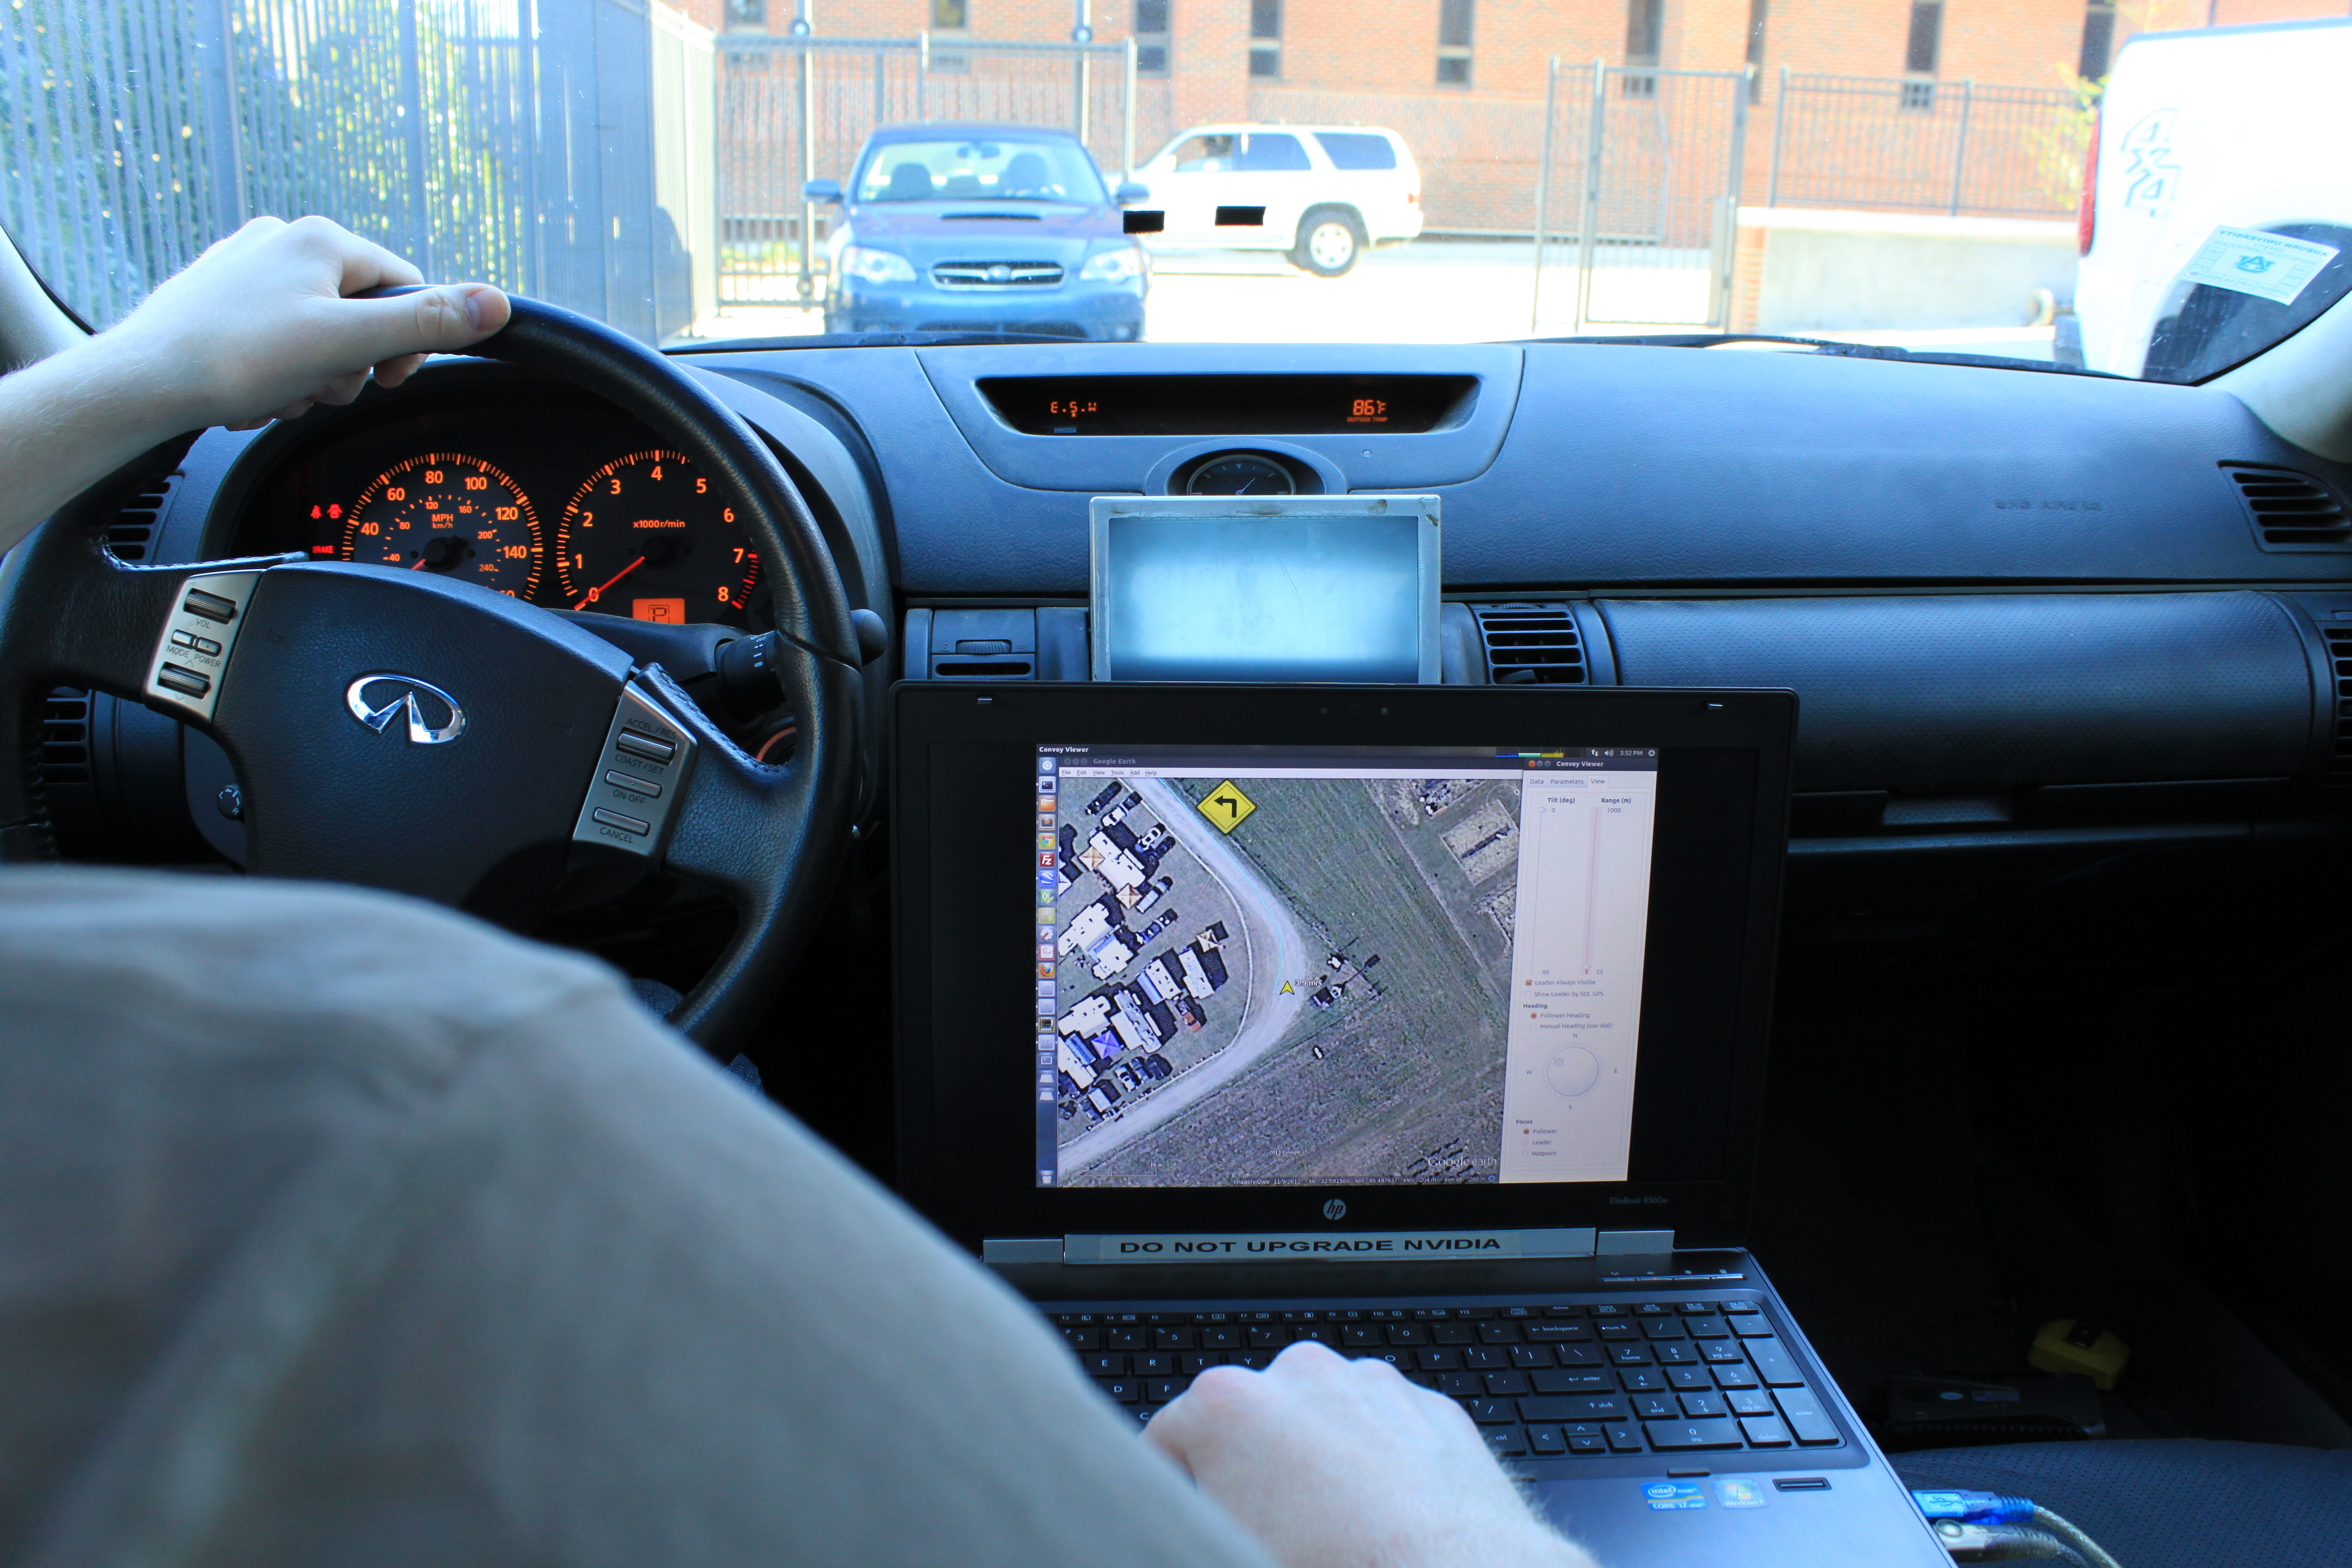
\includegraphics[width=4in] {../graphics/driver_view.jpg}
        \caption{View from the driver's seat} \label{fig:driver_view}
      \end{figure}
    \end{frame}

  \subsection{}



\end{document}